% A skeleton file for producing Computer Engineering reports
% https://kgcoe-git.rit.edu/jgm6496/KGCOEReport_template

\documentclass[CMPE]{KGCOEReport}

% The following should be changed to represent your personal information
\newcommand{\classCode}{CMPE 160}  % 4 char code with number
\newcommand{\name}{Andrei Tumbar}
\newcommand{\LabSectionNum}{4}
\newcommand{\LabInstructor}{Mr.\ Byers}	% The slash is to tell LaTeX that the period is between words
												% not sentences so it spaces correctly. It won't appear in the
												% final pdf
\newcommand{\TAs}{Sam Myers \\ Kobe Balin \\ Georgi Thomas}
\newcommand{\LectureSectionNum}{1}
\newcommand{\LectureInstructor}{Mr.\ Cliver}
\newcommand{\exerciseNumber}{7}
\newcommand{\exerciseDescription}{Sequential Circuit Elements}
\newcommand{\dateDone}{February 27th}
\newcommand{\dateSubmitted}{March 26th}

\graphicspath{{./lab7_media/}}

\usepackage{circuitikz}
\usepackage{tikz}
\usepackage{multirow}
\usepackage{titlesec}
\usepackage{float}
\usepackage{pgfplots, pgfplotstable}
\usepackage{lmodern}
\usepackage{siunitx}
\usepackage{subcaption}

\usepackage[usestackEOL]{stackengine}
\usepackage{scalerel}

\usepackage{kmap}
\usepackage[T1]{fontenc}

\usepackage{amsmath}

\def\lbar#1{\ThisStyle{%
  \setbox0=\hbox{$\SavedStyle#1$}%
  \stackengine{2.2\LMpt}{$\SavedStyle#1$}{\rule{\wd0}{0.1\LMpt}}{O}{c}{F}{F}{S}%
}}

\ctikzset{bipoles/not port/circle width=.4}
\ctikzset{tripoles/american xor port/height/.initial=.4}
\ctikzset{tripoles/american xor port/width/.initial=.6}

\DeclareFontFamily{U}{mathx}{\hyphenchar\font45}
\DeclareFontShape{U}{mathx}{m}{n}{ <-> mathx10 }{}
\DeclareSymbolFont{mathx}{U}{mathx}{m}{n}
\DeclareFontSubstitution{U}{mathx}{m}{n}
\DeclareMathAccent{\widebar}{\mathalpha}{mathx}{"73}

\makeatletter
\newcommand{\cwidebar}[2][0]{{\mathpalette\@cwidebar{{#1}{#2}}}}
\newcommand{\@cwidebar}[2]{\@cwideb@r{#1}#2}
\newcommand{\@cwideb@r}[3]{%
  \sbox\z@{$\m@th\mkern-#2mu#3\mkern#2mu$}%
  \widebar{\box\z@}%
}
\makeatother

\begin{document}
\maketitle

\section*{Abstract}
In this laboratory exercise a D flip-flop was created using two D-latches. This circuit configuration allows the resultant output value to only change on a clock edge. By implementing two D-latches with active-low enable, they were connected together to create the D flip-flop. Modelsim was used to simulate the design created in Quartus. Finally, the circuit was implemented on a breadboard and the clock signal was created using a $1\,Hz$ wave generator.

\section*{Design Methodology}

A D-latch is a circuit that can store boolean values and load new values. For this functionality, three actions must be implemented. \texttt{SET}, \texttt{RESET}, and \texttt{HOLD} are needed. \texttt{SET} and \texttt{RESET} are used to load the value 1 or 0 into the latch. \texttt{HOLD} will keep the previous value constant.

\begin{table}[h!]
\renewcommand{\arraystretch}{1.2}
\setlength{\tabcolsep}{12pt}
\caption{Function table for low enable D-latch}
\begin{center}
\begin{tabular}{|c|c||c|c|}
\hline
En & D & Q & Qn\\\hline
0 & 0 & 0 & 1\\\hline
0 & 1 & 1 & 0\\\hline
1 & X & $Q_0$ & $\widebar{Q_0}$\\\hline

\end{tabular}
\end{center}
\label{tab:dlatch}
\end{table}

Table \ref{tab:dlatch} shows the latch with a two input function. Because this D-latch is active-low enable, when the enable signal is low, Q takes on the value of D. When the enable is high, Q keeps the old value. This latch is asynchronous meaning that the Q value will change immediatly if the enable is low.

\begin{figure}[h!]
	\centering
	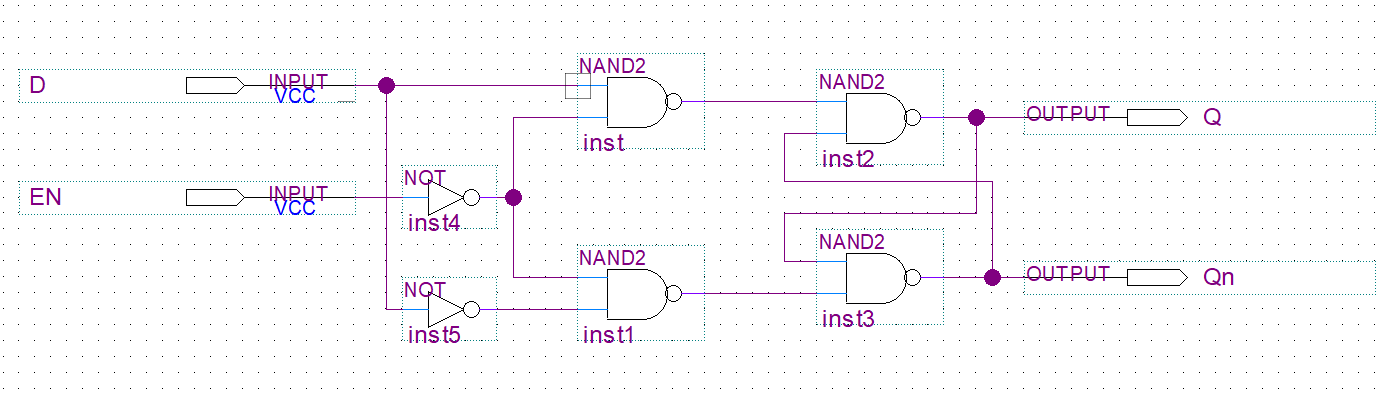
\includegraphics[width=\textwidth]{schematic1}
	\caption{D-latch circuit schematic}
	\label{fig:dlatch-schem}
\end{figure}

Figure \ref{fig:dlatch-schem} is a circuit schematic of the two-input D-latch described in Table \ref{tab:dlatch}. There is an inverter placed after the enable input to cause the latch to be active low.

To create a clock sensitive and synchronous D flip-flop, two D-latches must be used. By using two latches and inverting the enable signal used on the second one, the time delay between the two enables will cause the resultant value to only change on a clock edge.

\begin{table}[h!]
\renewcommand{\arraystretch}{1.2}
\setlength{\tabcolsep}{12pt}
\caption{Rising edge-triggered D flip-flop}
\begin{center}
\begin{tabular}{|c|c||c|c|}
\hline
clk & D & Q & Qn\\\hline
$\uparrow$ & 0 & 0 & 1\\\hline
$\uparrow$ & 1 & 1 & 0\\\hline
otherwise  & X & $Q_0$ & $\widebar{Q_0}$\\\hline

\end{tabular}
\end{center}
\label{tab:dflipflop}
\end{table}

Table \ref{tab:dflipflop} is very similar to Table \ref{tab:dlatch} in that the resultant values of Q and Qn are the same. However, Q only changes on a rising edge of the enable/clock signal.

\begin{figure}[h!]
	\centering
	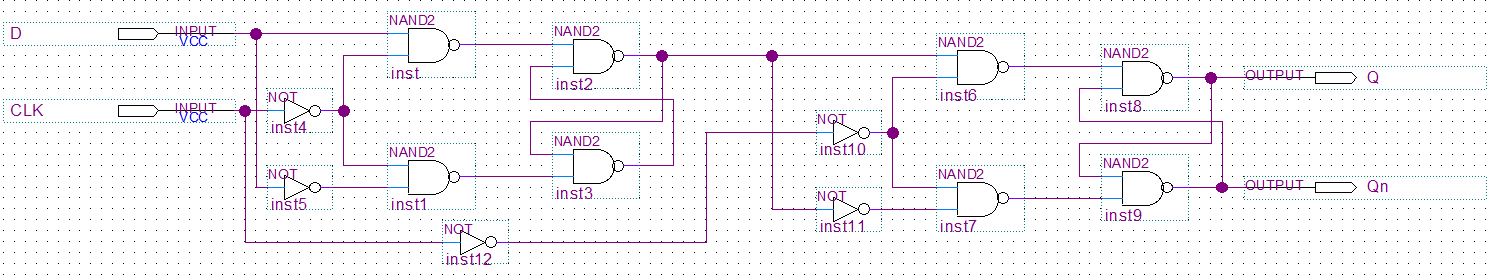
\includegraphics[width=\textwidth]{schematic2}
	\caption{D flip-flop circuit schematic}
	\label{fig:dflipflop-schem}
\end{figure}

Figure \ref{fig:dflipflop-schem} shows the circuit configuration of the D flip-flop using two D-latches. The output of the first latch is sent to the input of the second latch. The \texttt{CLK} signal is inverted and sent to the enable of the second D-latch. The time delay on the inverter of the \texttt{CLK} will cause the output, Q, to change only when the clock value is rising.

\section*{Results and Analysis}

After the D-latch and flip-flop were designed in Quartus, a simulation in Modelsim was performed.

\begin{figure}[h!]
	\centering
	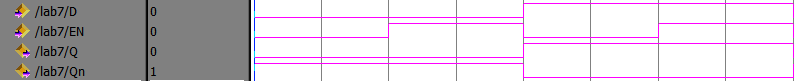
\includegraphics[width=\textwidth]{part1}
	\caption{D-latch simulation}
	\label{fig:dlatch-sim}
\end{figure}

Figure \ref{fig:dlatch-sim} shows the results of the a modelsim simulation run with the D-latch circuit. When the \texttt{EN} signal was low, \texttt{Q} took the value of \texttt{D}. When the \texttt{EN} is high, \texttt{D} is ignored and \texttt{Q} is held to the current value. This is exactly how the D-latch was described in the previous section.\\

The D flip-flop was also simulated in this exercise. The enable signal however was changed to a clock signal.\pagebreak

\begin{figure}[h!]
	\centering
	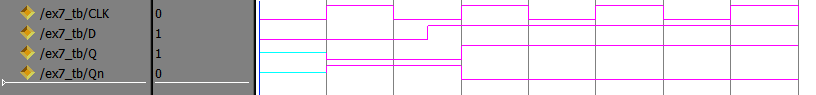
\includegraphics[width=\textwidth]{part2}
	\caption{D flip-flop simulation}
	\label{fig:dflipflop-sim}
\end{figure}

The change on the D signal in Figure \ref{fig:dflipflop-sim} was placed offset to the \texttt{CLK} changes as to show a typical occurance in this circuit. Also, if the input signal, \texttt{D} were to change too closely to the clock edge, the circuit would enter a metastasis in which either 0 or 1 could result. The results of this simulation were as expected. The value of \texttt{Q} is unknown before the first clock edge therefore depicted with a line inbetween the logical 1 and 0 values. On every rising clock edge \texttt{Q} takes on the value of \texttt{D}.\\

After the simulations were completed, two D-latches were implemented and tested on a breadboard. After the integrity of the D-latches were verified, the two latches were combined to create a D-flipflop.

\begin{figure}[h!]
	\centering
	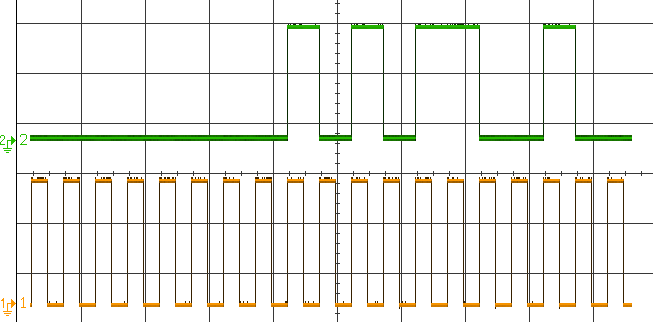
\includegraphics[width=\textwidth]{scope_p0.png}
	\caption{D flip-flop oscilloscope capture.}
	\label{fig:dosc}
\end{figure}

Figure \ref{fig:dosc} shows the results of the oscilloscope capture of from the D flip-flop implementation on the breadboard. Probe 1 was placed on the clock signal which shows a $1\,Hz$ square wave generated by the square wave function on the oscilloscope. Probe 2 was placed on the output signal. The input signal was arbitrarily controlled to  test the integrity of the circuit. The results here correctly depict the functionality of the D flip-flop because value changes on the output only occur on the rising edge of the clock signal.

\section*{Conclusion}

In this laboratory exercise, a D-latch and D flip-flop were designed and simulated and later built on a breadboard. The use of a clock was made clear in designing the D flip-flop as the time delay on the inverter between the two D-latches allows for the output value to update only on a rising clock edge. The resulting simulations and breadboard experiment were successful in that they produced the desired output described.

\section*{Questions}

\begin{enumerate}

\item Design a falling edge-triggered D flip-flop using D latches with active-low enable.

\begin{figure}[h!]
	\centering
	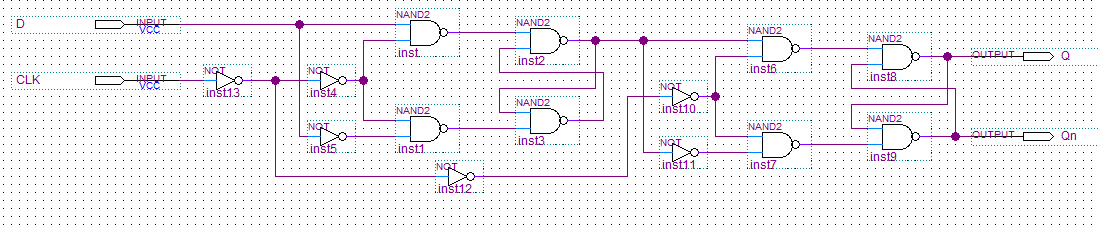
\includegraphics[width=\textwidth]{q1.png}
	\caption{Falling edge triggered D flip-flop with active low enabled D latches}
	\label{fig:q1}
\end{figure}

The only different between the falling edge-triggered D flip-flop and the rising edge is the inverter directly after the \texttt{CLK} signal. This will flip the clock and make all of the original rising edges be falling edges.

\item The 74LS175 is a quad D flip-flop IC with an asynchronous master reset pin. The maximum time needed for the MR (master reset) is $30\,ns$. The maximum time to output change after the rising clock edge is $25\,ns$. The minimum setup time before the rising clock edge is $20\,ns$. Finally the minimum hold time after the rising clock edge is $5\,ns$.

\end{enumerate}
\end{document}
